\section{Second Member}
This is the section dedicated to one of the team members, and it should be written individually . It can include a range of things; first subsection is a space for you to point out the strengths and weaknesses of the module, including complaints about the module coordinator Max Wilson. The second section should have a selfie image with Max! The last part of it is the most important one. You will need to write a paragraph about what you have learned in this module. You can write it in \textbf{Bold} if you want or you can use other fonts. 



Please do not forget:
\begin{itemize}
	\item First paragraph should have your comments about the module
	\item Second one, a selfie img with Max
	\item Last one, what you learned in this module.
\end{itemize}

\subsection{Comments about the module}
This module was a little boring due to the content size of the presentations. However, I found working in teams a good aspect to get ready for the real world application and I like the fact that we were able to go through the whole of the software engineering process instead of just the implementation. During this term, Max was able to deliver the content very quickly while still being able to ensure students have the correct understanding of each lecture. In addition, Max Wilson was very experienced and no uncertainty when answering questions. I feel like more  time could be given to ensure we are exam ready, as I have feel we aren't testing the lecture notes to exam application. Lastly, there is a little bit too much reading content for me to handle in this module.

\subsection{Selfie with Max}

Please refer below to amazing selfie.

\begin{figure}[h]
\caption{Selfie with Max}
\centering
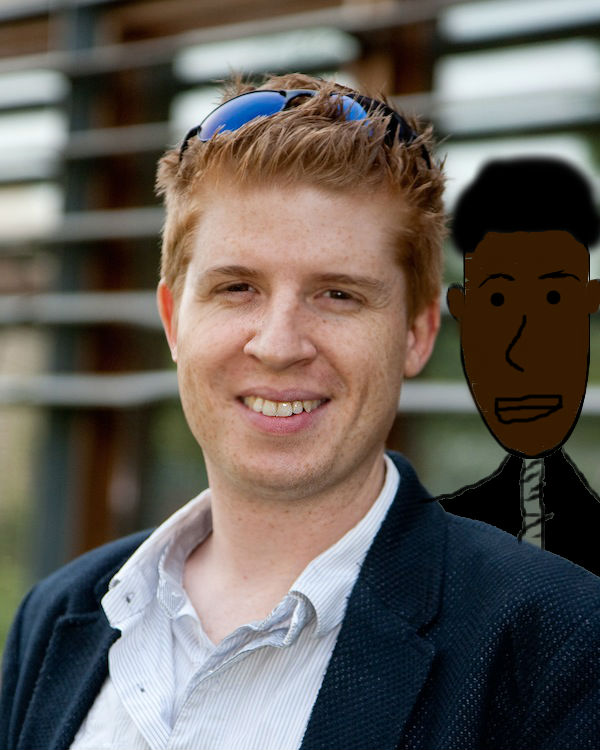
\includegraphics[width=0.5\textwidth]{maxSelfie.jpg}
\label{fig:selfie}
\end{figure}

% My selfie with Max is in  Figure~\ref{fig:selfie}.

\subsection{What I have learned in this module}
What I have learnt in this module is how to prepare for the real world by going through the software cycle in detail with the addition of working in teams! In addition, I have learnt how different components work together such as latex and Git. Finally, I have learnt all the visual representations to show the clients what we are deciding to make for them. 

